\documentclass[11pt]{article}

\usepackage[a4paper,margin=1in]{geometry}
\usepackage[T1]{fontenc}
\usepackage[utf8]{inputenc}
\usepackage{amsmath,amssymb,mathtools}
\usepackage{graphicx}
\usepackage{booktabs}
\usepackage{tabularx}
\usepackage{array}
\usepackage{subcaption}
\usepackage{hyperref}
\usepackage{enumitem}

\hypersetup{
    colorlinks=true,
    linkcolor=blue,
    citecolor=blue,
    urlcolor=blue
}

\newcommand{\UL}{\mathrm{UL}}
\newcommand{\DL}{\mathrm{DL}}
\newcommand{\F}{\mathbf{F}}
\newcommand{\Hc}{\mathbf{H}}
\newcommand{\Sig}{\mathbf{\Sigma}}
\newcommand{\norm}[1]{\left\lVert #1 \right\rVert}

\title{Current Uplink--Downlink Method Report\\for Finite-Blocklength Latency Experiments}
\author{}
\date{June 22, 2026}

\begin{document}

\maketitle

\begin{abstract}
This report is a dated rewrite of the legacy combined uplink/downlink document. Its purpose is not to restate every exploratory derivation, but to document the current cleaned method set, explain how each method trains and tests, and summarize only the artifacts that are actually present today. Where a method implementation exists but a finalized comparable result artifact is missing, the method is still documented and the missing status is stated explicitly rather than replaced by guessed numbers.
\end{abstract}

\section{Scope and Artifact Policy}
The cleaned experiment folder now contains six main method paths:
\begin{enumerate}[leftmargin=1.5em]
    \item uplink convergence-per-sweep baseline,
    \item uplink Monte Carlo precoder net,
    \item uplink Monte Carlo shared-beam precoder net,
    \item downlink convergence-per-sweep baseline,
    \item downlink Monte Carlo precoder net, and
    \item downlink Monte Carlo shared-beam precoder net.
\end{enumerate}

This rewrite follows one rule:
\begin{quote}
\textbf{Use current artifacts where they exist; otherwise document the method and state that the matching current artifact is missing or incomplete.}
\end{quote}

That rule matters because the legacy report folder still contains older illustrative figures, but it does not contain a complete, current, cleaned result set for every method. In particular:
\begin{itemize}[leftmargin=1.5em]
    \item the current cleaned uplink convergence baseline artifacts are missing from the report workspace,
    \item the current cleaned shared-beam report artifacts are not finalized in a comparable form, and
    \item the current per-\(n_{k,\ell}\) Monte Carlo artifacts are available and can be summarized quantitatively.
\end{itemize}

\section{Shared Problem View}
Across both links, user \(k\) carries payload \(B_k\), target reliability \(\varepsilon_k\), power budget \(P_k\), symbol rate \(f_{s,k}\), and coherence-limited maximum blocklength \(T_k\). If the payload is transmitted over scheduled blocks indexed by \(\ell\), then the latency of user \(k\) is
\begin{equation}
\tau_k = \frac{1}{f_{s,k}} \sum_{\ell} n_{k,\ell}.
\end{equation}

All methods therefore try to reduce total latency through better choices of
\begin{equation}
\{B_{k,\ell}, n_{k,\ell}, \F_{k,\ell}\},
\end{equation}
subject to finite-blocklength feasibility
\begin{equation}
\frac{B_{k,\ell}}{n_{k,\ell}} \le R_{k,\ell}^{(\UL/\DL)}.
\end{equation}

The main difference between the methods is not the latency definition but the \emph{way} the precoder is produced:
\begin{itemize}[leftmargin=1.5em]
    \item online convergence methods optimize the precoder directly during test-time scheduling,
    \item Monte Carlo per-\(n_{k,\ell}\) methods train a precoder net whose input includes \(n_{k,\ell}\),
    \item Monte Carlo shared-beam methods train a precoder net once per scenario and reuse the same beam across a candidate \(n_{k,\ell}\) grid.
\end{itemize}

\section{Method Inventory}
\begin{table}[ht]
\centering
\small
\caption{Current cleaned method inventory}
\renewcommand{\arraystretch}{1.15}
\begin{tabularx}{\textwidth}{>{\raggedright\arraybackslash}p{0.12\textwidth} >{\raggedright\arraybackslash}p{0.23\textwidth} X X}
\toprule
Link & Method & Training idea & Testing idea \\
\midrule
Uplink & Convergence per sweep & No offline training. Optimize each user block directly at test time. & For each user, create blocks as needed, optimize the block precoder, then shrink \(n_{k,\ell}\) greedily while feasibility holds. \\
Uplink & Monte Carlo precoder net & One net per user. Dataset samples are \((H_{k,\ell}, n_{k,\ell}, \Sig_{k,\ell}, \varepsilon_k)\). Train with a Lagrangian finite-blocklength objective. & At test time, the user net predicts a fresh precoder for each candidate \(n_{k,\ell}\). \\
Uplink & Monte Carlo shared beam & One net per user. Dataset scenarios are \((H_{k,\ell}, \Sig_{k,\ell}, \varepsilon_k)\) with a candidate \(n_{k,\ell}\) grid. & Predict one beam once, then reuse it across the \(n_{k,\ell}\) search. \\
Downlink & Convergence per sweep & No offline training. Joint online block optimization over active users. & In each block, first converge the active-user precoders jointly, then allocate bits and shrink \(n_{k,\ell}\). \\
Downlink & Monte Carlo precoder net & One net per user, trained jointly. Dataset cases are \((H_{\ell}, n_{k,\ell}, a_{\ell}, \Sig_{k,\ell}, \varepsilon_k)\). & In each block, each active user net predicts its beam using the current \(n_{k,\ell}\), then the scheduler allocates bits. \\
Downlink & Monte Carlo shared beam & One net per user, trained jointly. Dataset cases are \((H_{\ell}, a_{\ell}, \Sig_{k,\ell}, \varepsilon_k)\) plus candidate \(n\)-levels. & Predict one beam per active user once, then reuse the same beams while testing multiple \(n_{k,\ell}\) values. \\
\bottomrule
\end{tabularx}
\end{table}

\section{Uplink Methods}
\subsection{Convergence per Sweep Baseline}
\paragraph{Method idea.}
This is the direct online baseline. There is no offline dataset and no trained network. For a given user and a given block, the solver alternates between improving the precoder and checking which finite-blocklength \(n_{k,\ell}\) is feasible. If the remaining payload does not fit in one block, the algorithm creates another block and repeats.

\paragraph{Training idea.}
There is no training stage.

\paragraph{Testing idea.}
Testing is the full algorithm: initialize a block, converge the precoder for that block, greedily shrink \(n_{k,\ell}\) while the selected bit load stays feasible, commit the block, and continue until the user payload is fully served.

\paragraph{Artifact status.}
The dated report folder still contains older uplink illustrative figures, but the current cleaned baseline result artifact that should match the cleaned experiment folder is missing here. For that reason, this report does \emph{not} quote a new quantitative baseline table for uplink convergence, and instead documents the method only.

\subsection{Monte Carlo Precoder Net}
\paragraph{Precoder-net input.}
The current cleaned uplink Monte Carlo net is blocklength-aware:
\begin{equation}
\F_{k,\ell} = f_{\theta_k}(H_{k,\ell}, n_{k,\ell}, \Sig_{k,\ell}, \varepsilon_k).
\end{equation}
Each user has its own net, but the net is shared across that user's training samples.

\paragraph{Training idea.}
The available seed-3 artifact uses train seeds \(0,1,2\). The dataset contains \(864\) total training samples, with \(288\) samples per user and four channel blocks per seed. Each sample is one
\[
(\text{seed}, \text{user}, \text{block}, n_{k,\ell})
\]
item, and the cleaned report artifact states that the minimum required transmitted bits per sample is fixed to \(1\).

The important point is that the training loss is \emph{not} MSE to an expert label. It is a direct Lagrangian finite-blocklength objective. The available training summary reports:
\begin{itemize}[leftmargin=1.5em]
    \item final average user rate \(= 13.8813\),
    \item final average Lagrangian \(= -13.8349\),
    \item final average rate violation \(= 0.0779\),
    \item final average power violation \(\approx 10^{-6}\),
    \item train-eval latency reduction \(= 18.35\%\) on the first training seed.
\end{itemize}

\paragraph{Testing idea.}
At test time, the scheduler still follows the greedy payload-serving logic. The difference is that the precoder itself comes from the trained user net, and a \emph{fresh} beam is predicted for each candidate \(n_{k,\ell}\) during the search.

\paragraph{Observed behavior from the available cleaned artifact.}
The seed-3 testing summary shows modest latency improvement but weaker synchronization behavior:
\begin{itemize}[leftmargin=1.5em]
    \item total latency reduction \(= 8.82\%\),
    \item asynchronality reduction \(= -50.0\%\), meaning pairwise latency spread increased,
    \item final average SINR improved only slightly from \(-3.2572\) dB to \(-3.2132\) dB.
\end{itemize}

\begin{figure}[ht]
\centering
\begin{subfigure}[t]{0.48\textwidth}
    \centering
    
\includegraphics[width=\textwidth]{figures/current_results/uplink_mc/latency_comparison.png}
    \caption{Latency comparison}
\end{subfigure}
\hfill
\begin{subfigure}[t]{0.48\textwidth}
    \centering
    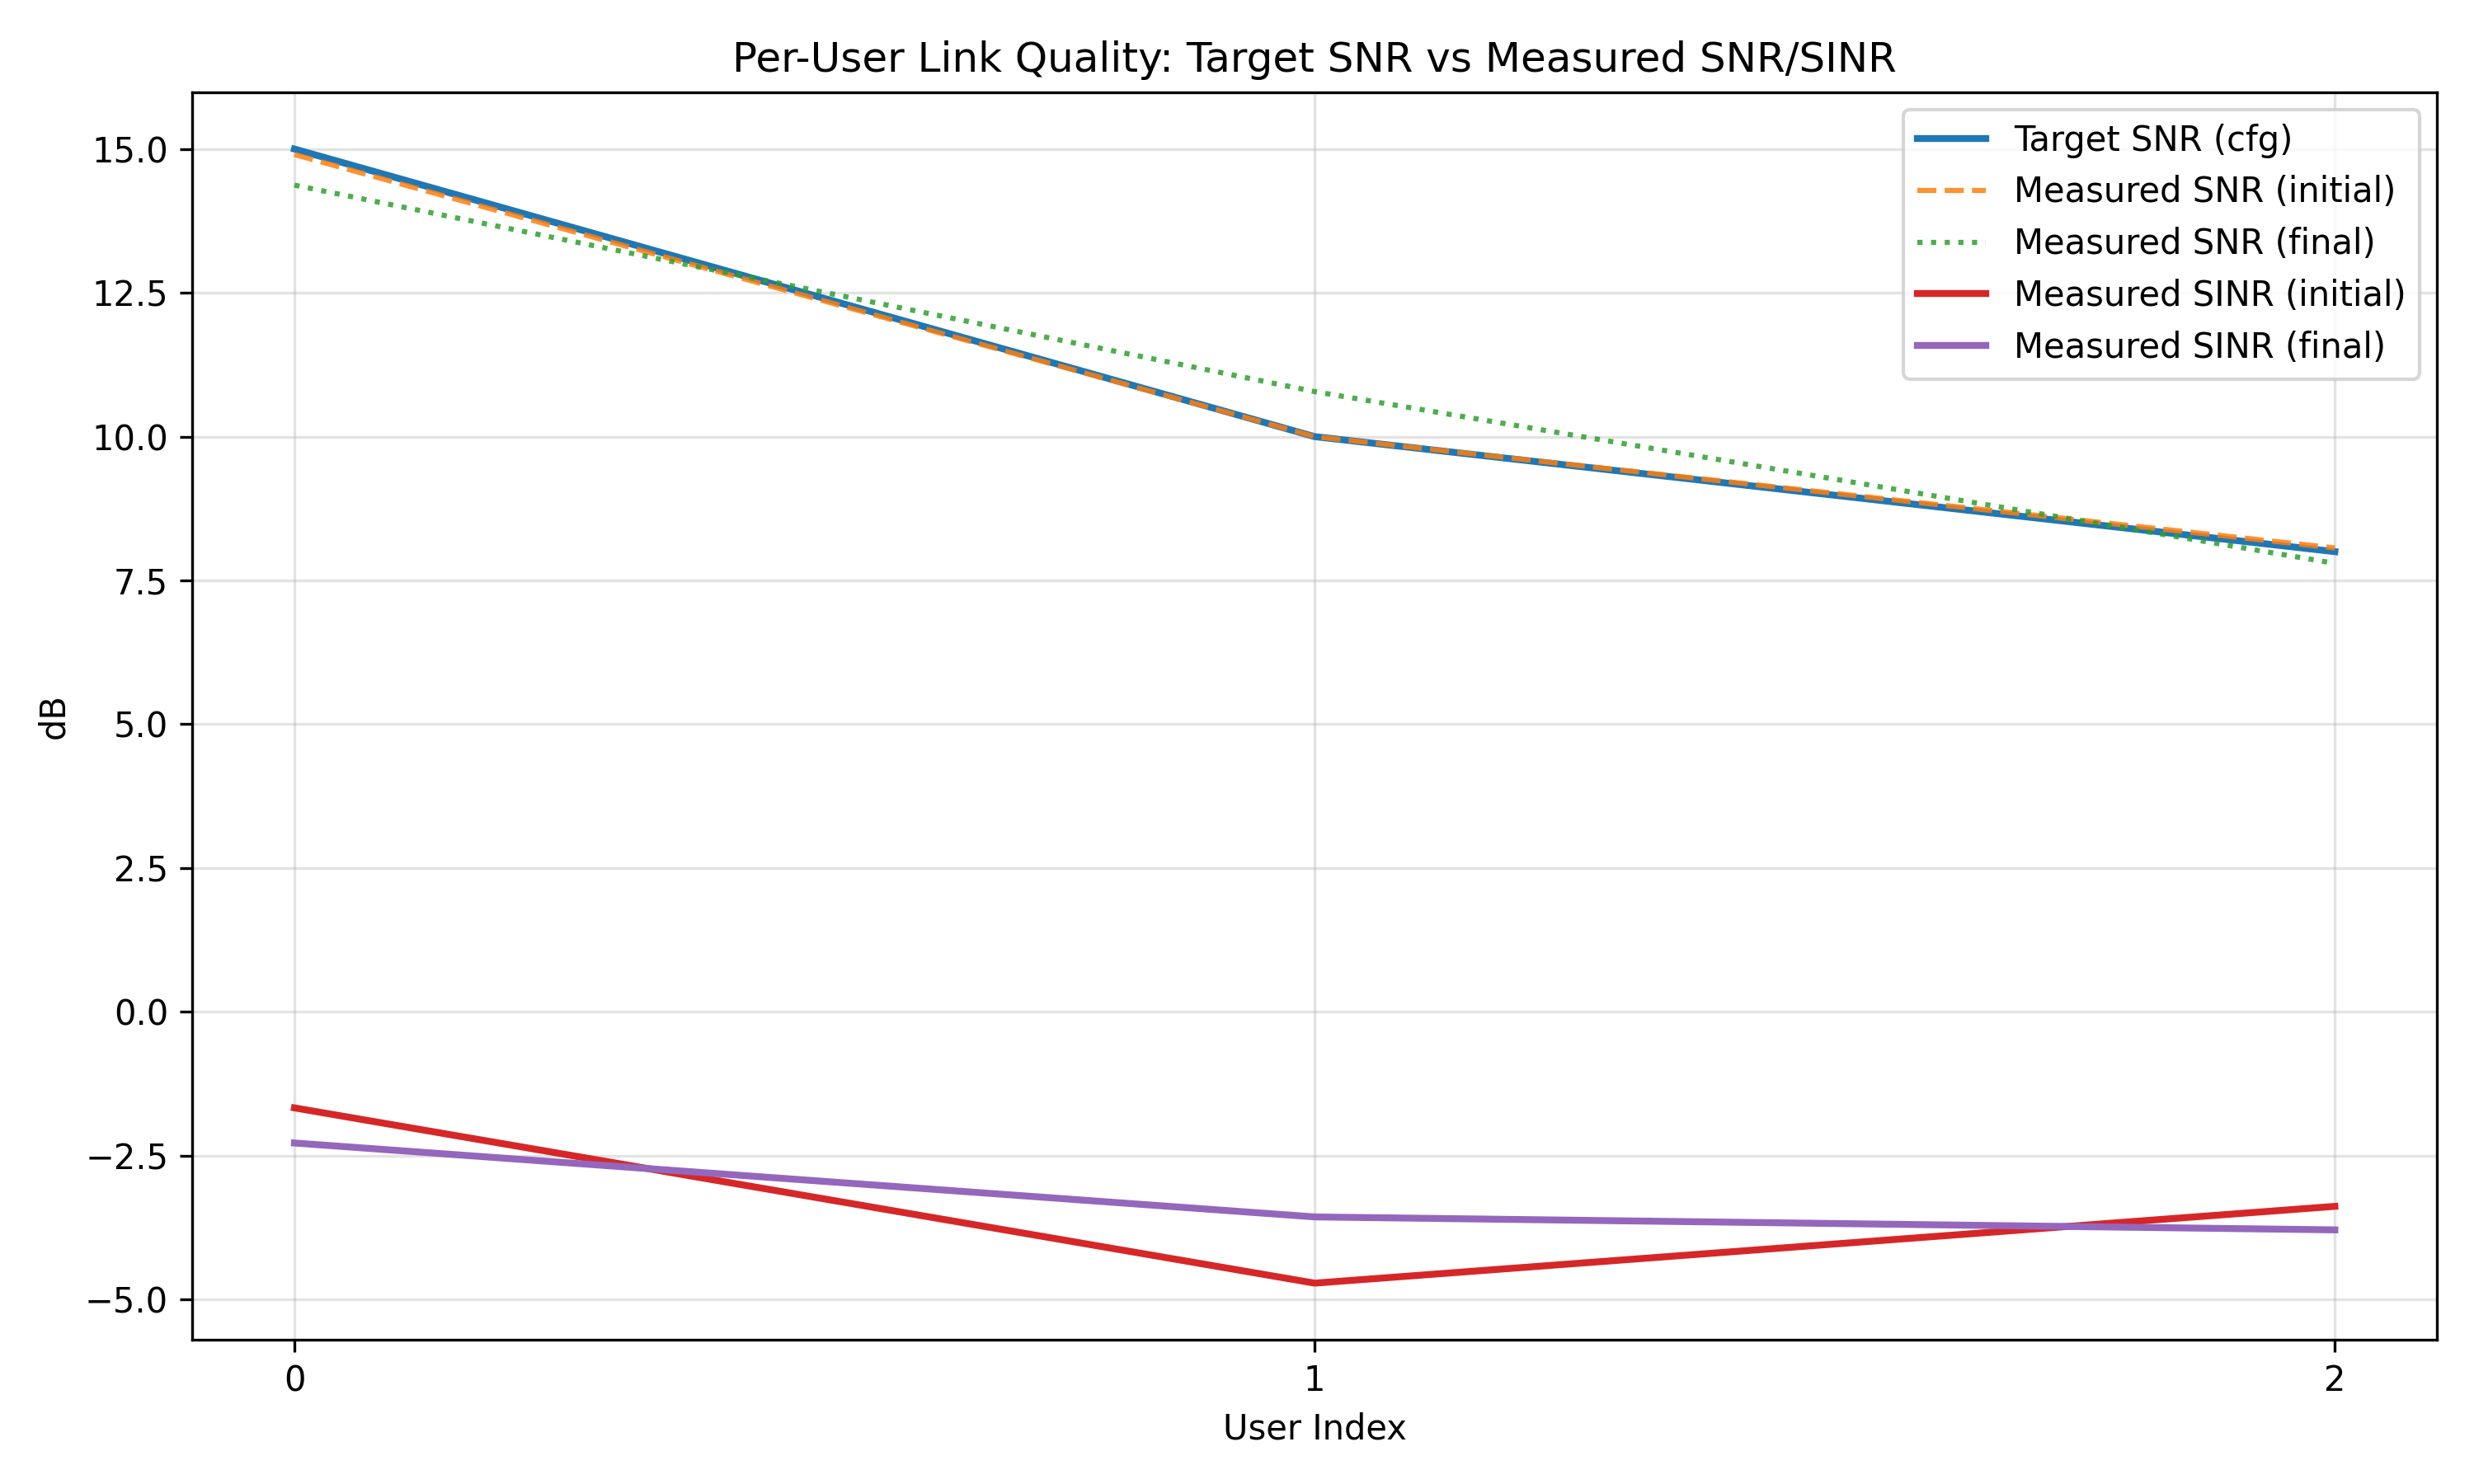
\includegraphics[width=\textwidth]{figures/current_results/uplink_mc/link_quality_comparison.png}
    \caption{Link-quality comparison}
\end{subfigure}
\caption{Available current uplink Monte Carlo test figures from the cleaned seed-3 artifact.}
\label{fig:uplink-mc-current}
\end{figure}

\subsection{Monte Carlo Shared Beam}
\paragraph{Precoder-net input.}
The shared-beam uplink net removes \(n_{k,\ell}\) from the input:
\begin{equation}
\F_{k,\ell} = f_{\theta_k}(H_{k,\ell}, \Sig_{k,\ell}, \varepsilon_k).
\end{equation}

\paragraph{Training idea.}
Each scenario contains a channel block and a candidate \(n_{k,\ell}\) grid. The net predicts one beam once, and that same beam is evaluated across all candidate \(n_{k,\ell}\) values. The training objective is therefore an average shared-beam finite-blocklength rate over the \(n\)-grid, rather than a fresh-beam objective at every \(n\).

\paragraph{Testing idea.}
Testing follows the same logic: one beam prediction per scenario, then reuse of that beam while scanning candidate \(n_{k,\ell}\) values until the smallest feasible value is found.

\paragraph{Artifact status.}
The method implementation exists and a shared-beam report folder was created, but this report workspace does not contain a finalized, comparable cleaned result package for the seed-3 uplink shared-beam run. Therefore the method is documented here but not included in the quantitative comparison table.

\section{Downlink Methods}
\subsection{Convergence per Sweep Baseline}
\paragraph{Method idea.}
The cleaned downlink baseline is a joint online scheduler. In each common block, the active-user set is formed from users with remaining payload. The scheduler then updates the active-user precoders jointly until the block converges, and \emph{only after that} allocates bits and shrinks the chosen \(n_{k,\ell}\).

\paragraph{Training idea.}
There is no offline training stage.

\paragraph{Testing idea.}
Testing is the algorithm itself. Two objective settings are available in the current artifacts:
\begin{itemize}[leftmargin=1.5em]
    \item \texttt{user\_rate}: a user-wise greedy objective,
    \item \texttt{weighted\_sum\_rate}: a stronger coupled objective that still uses the same online scheduling structure.
\end{itemize}

\paragraph{Observed behavior from available cleaned artifacts.}
Two current seed-3 artifacts are available:
\begin{itemize}[leftmargin=1.5em]
    \item \texttt{user\_rate}: total latency reduction \(= 84.46\%\), final average SINR \(= 4.73\) dB,
    \item \texttt{weighted\_sum\_rate}: total latency reduction \(= 90.89\%\), final average SINR \(= 7.65\) dB.
\end{itemize}
Among the available downlink artifacts, the weighted-sum-rate objective is the strongest baseline in this report.

\begin{figure}[ht]
\centering
\begin{subfigure}[t]{0.48\textwidth}
    \centering
    
\includegraphics[width=\textwidth]{figures/current_results/downlink_conv_weighted/latency_comparison.png}
    \caption{Latency comparison}
\end{subfigure}
\hfill
\begin{subfigure}[t]{0.48\textwidth}
    \centering
    
\includegraphics[width=\textwidth]{figures/current_results/downlink_conv_weighted/optimization_history.png}
    \caption{Optimization history}
\end{subfigure}
\caption{Available current downlink convergence-per-sweep figures for the \texttt{weighted\_sum\_rate} objective.}
\label{fig:downlink-conv-current}
\end{figure}

\subsection{Monte Carlo Precoder Net}
\paragraph{Precoder-net input.}
The current cleaned downlink Monte Carlo net is blocklength-aware and interference-aware:
\begin{equation}
\F_{k,\ell} = f_{\theta_k}(H_{\ell}, n_{k,\ell}, a_{\ell}, \Sig_{k,\ell}, \varepsilon_k),
\end{equation}
where \(H_{\ell}\) is the full block context and \(a_{\ell}\) is the active-user mask.

\paragraph{Training idea.}
The training dataset is joint rather than user-independent. One training case is a
\[
(\text{seed}, \text{block}, \text{active mask})
\]
item, and the current seed-3 artifact reports:
\begin{itemize}[leftmargin=1.5em]
    \item \(720\) total training cases,
    \item case split \(240/240/240\) across train seeds \(0,1,2\),
    \item active-user-case counts \([360,396,432]\) for users \(0,1,2\).
\end{itemize}

The objective is again not MSE imitation. It is a direct Lagrangian objective built from sum finite-blocklength rate, rate feasibility, and power feasibility. The current cleaned artifact reports:
\begin{itemize}[leftmargin=1.5em]
    \item final average training sum rate \(= 20.4893\),
    \item final average user rate \(= 12.3861\),
    \item final feasible training-case fraction \(= 1.0\),
    \item zero final average rate violation,
    \item \(7749\) curriculum reduction events.
\end{itemize}

\paragraph{Testing idea.}
At test time, the active users in a block each predict their beam using the current \(n_{k,\ell}\), active mask, and interference input. The scheduler then allocates bits and performs the usual greedy \(n_{k,\ell}\) shrink rule.

\paragraph{Observed behavior from the available cleaned artifact.}
The most important finding is that stable training did \emph{not} translate into stronger test-time scheduling than the online baseline:
\begin{itemize}[leftmargin=1.5em]
    \item total latency changed from \(0.0768\) s to \(0.0798\) s, which is a \(-3.91\%\) reduction, i.e.\ a regression,
    \item asynchronality changed by \(-13.79\%\), again a regression,
    \item average SINR improved only from \(-3.5566\) dB to \(-2.8353\) dB.
\end{itemize}
So the current downlink Monte Carlo training pipeline is numerically stable but not yet competitive with the online convergence baseline.

\begin{figure}[ht]
\centering
\begin{subfigure}[t]{0.48\textwidth}
    \centering
    
\includegraphics[width=\textwidth]{figures/current_results/downlink_mc/latency_comparison.png}
    \caption{Latency comparison}
\end{subfigure}
\hfill
\begin{subfigure}[t]{0.48\textwidth}
    \centering
    
\includegraphics[width=\textwidth]{figures/current_results/downlink_mc/optimization_history.png}
    \caption{Optimization history}
\end{subfigure}
\caption{Available current downlink Monte Carlo test figures from the cleaned seed-3 artifact.}
\label{fig:downlink-mc-current}
\end{figure}

\subsection{Monte Carlo Shared Beam}
\paragraph{Precoder-net input.}
The shared-beam downlink net removes \(n_{k,\ell}\) from the input:
\begin{equation}
\F_{k,\ell} = f_{\theta_k}(H_{\ell}, a_{\ell}, \Sig_{k,\ell}, \varepsilon_k).
\end{equation}

\paragraph{Training idea.}
Each training case stores the full block context, active-user mask, and a joint \(n\)-level grid. The user nets predict one beam each, and those fixed beams are reused across the candidate \(n_{k,\ell}\) levels while the objective averages the resulting sum finite-blocklength rates.

\paragraph{Testing idea.}
Testing follows the same shared-beam philosophy. For a block, the active users predict one beam each, the interference environment is evaluated with those beams fixed, and the scheduler reuses them during the greedy \(n_{k,\ell}\) search.

\paragraph{Artifact status.}
The method is implemented and the report folder structure exists, but this dated rewrite does not have a finalized current cleaned shared-beam result package that is comparable to the baseline and per-\(n\) Monte Carlo seed-3 artifacts. The method is therefore documented but excluded from numerical ranking.

\section{Available Quantitative Snapshot}
\begin{table}[ht]
\centering
\small
\caption{Method-by-method status using only currently available artifacts}
\renewcommand{\arraystretch}{1.15}
\begin{tabularx}{\textwidth}{>{\raggedright\arraybackslash}p{0.22\textwidth} >{\raggedright\arraybackslash}p{0.16\textwidth} >{\centering\arraybackslash}p{0.14\textwidth} >{\centering\arraybackslash}p{0.14\textwidth} X}
\toprule
Method & Artifact status & Total latency reduction & Asynchronality reduction & Comment \\
\midrule
Uplink convergence per sweep & Missing current cleaned artifact & n/a & n/a & Method documented, but no matching current quantitative package in this workspace. \\
Uplink Monte Carlo precoder net & Available & \(8.82\%\) & \(-50.0\%\) & Modest latency gain, but pairwise synchronization worsened. \\
Uplink Monte Carlo shared beam & Missing finalized artifact & n/a & n/a & Implementation exists; finalized comparable report artifact not available here. \\
Downlink convergence (\texttt{user\_rate}) & Available & \(84.46\%\) & \(73.40\%\) & Strong online baseline. \\
Downlink convergence (\texttt{weighted\_sum\_rate}) & Available & \(90.89\%\) & \(86.70\%\) & Best available downlink result in the current cleaned artifacts. \\
Downlink Monte Carlo precoder net & Available & \(-3.91\%\) & \(-13.79\%\) & Training is stable, but test-time scheduling underperforms the online baseline. \\
Downlink Monte Carlo shared beam & Missing finalized artifact & n/a & n/a & Implementation exists; finalized comparable report artifact not available here. \\
\bottomrule
\end{tabularx}
\end{table}

\begin{table}[ht]
\centering
\small
\caption{Available Monte Carlo training snapshots}
\renewcommand{\arraystretch}{1.15}
\begin{tabularx}{\textwidth}{>{\raggedright\arraybackslash}p{0.26\textwidth} >{\centering\arraybackslash}p{0.18\textwidth} >{\centering\arraybackslash}p{0.18\textwidth} X}
\toprule
Method & Dataset size & Final training metric & Interpretation \\
\midrule
Uplink Monte Carlo precoder net & \(864\) samples total, \(288\) per user & Avg.\ user rate \(= 13.8813\), avg.\ Lagrangian \(= -13.8349\) & User-wise offline training works numerically and improves train-eval latency, but test gains are limited. \\
Downlink Monte Carlo precoder net & \(720\) training cases, active-user-case counts \([360,396,432]\) & Avg.\ sum rate \(= 20.4893\), feasible fraction \(= 1.0\) & Joint training is numerically stable and fully feasible on the training set, but the learned scheduler does not yet beat the online baseline. \\
\bottomrule
\end{tabularx}
\end{table}

\section{What Is Missing}
This dated rewrite intentionally calls out the current gaps instead of hiding them:
\begin{enumerate}[leftmargin=1.5em]
    \item The current cleaned uplink convergence baseline result package is missing from the report workspace, so the baseline is described methodologically but not scored numerically here.
    \item The shared-beam methods are implemented on both links, but the report workspace does not yet contain finalized current artifacts that are directly comparable to the available seed-3 baseline and per-\(n\) Monte Carlo runs.
    \item The legacy report figures still exist in this folder, but they are not used as quantitative evidence when the matching cleaned artifact is missing.
\end{enumerate}

\section{Conclusion}
The main change in this rewrite is the viewpoint. The report is now organized around \emph{current methods and current artifacts}, not around older derivation branches.

The current evidence says the following:
\begin{itemize}[leftmargin=1.5em]
    \item uplink Monte Carlo training is working as an optimization routine, but the available test artifact shows only a modest latency gain and worse asynchronality,
    \item downlink online convergence remains the strongest available family, especially with the \texttt{weighted\_sum\_rate} objective,
    \item downlink Monte Carlo training is stable but is not yet competitive in test-time latency,
    \item the shared-beam methods are important new additions to the cleaned codebase, but this report can only document their design until finalized comparable artifacts are produced.
\end{itemize}

That makes this report useful in two ways: it records the exact training and testing ideas for every current method, and it also identifies which result packages still need to be generated before the full method comparison is complete.

\end{document}
